% 
% Modelo white-paper 
%
% Marcelo Pereira
%
% 
% e-mail: psnc4ards@gmail.com
%


\documentclass[
	% -- opções da classe memoir --
	article,			% indica que é um artigo acadêmico
	12pt,				% tamanho da fonte
	oneside,			% para impressão apenas no verso. Oposto a twoside
	a4paper,			% tamanho do papel. 
	% -- opções do pacote babel --
	%english,			% idioma adicional para hifenização
	brazil,				% o último idioma é o principal do documento
	english,
	sumario=tradicional
	]{abntex2}


% ---
% PACOTES
% ---

% ---
% Pacotes fundamentais 
% ---
\usepackage{lmodern}			% Usa a fonte Latin Modern
\usepackage[T1]{fontenc}		% Selecao de codigos de fonte.
\usepackage[utf8]{inputenc}		% Codificacao do documento (conversão automática dos acentos)
\usepackage{nomencl} 			% Lista de simbolos
\usepackage{color}				% Controle das cores
\usepackage{graphicx}			% Inclusão de gráficos
\usepackage{microtype} 			% Para melhorias de justificação
\usepackage{float}				% Para ajuste na posição de figuras e tabelas
\usepackage{tikz}
\usepackage{pgf}
\usepackage{adjustbox}
\usepackage{amsmath,amsthm,amsfonts,amssymb}
\definecolor{barblue}{RGB}{153,204,254}
\definecolor{groupblue}{RGB}{51,102,254}
\definecolor{linkred}{RGB}{165,0,33}

\usepackage{amsmath}
\usepackage{tikz}
\usepackage{mathdots}
\usepackage{yhmath}
\usepackage{cancel}
\usepackage{color}
\usepackage{siunitx}
\usepackage{array}
\usepackage{multirow}
\usepackage{amssymb}
\usepackage{gensymb}
\usepackage{tabularx}
\usepackage{booktabs}




% ---
		
% ---
% Pacotes adicionais, usados apenas no âmbito do Modelo Canônico do abnteX2
% ---
\usepackage{lipsum}				% para geração de dummy text
% ---
		
% ---
% Pacotes de citações
% ---
\usepackage[alf]{abntex2cite}	% Citações padrão ABNT
% ---

% ---
% Informações de dados para CAPA e FOLHA DE ROSTO
% ---
\titulo{Reactioon White Paper}
\autor{José Wilker,  \and Jonathas Figueiredo, \and Lucas Tonini}
\local{Brasil}
\data{} 
% ---

% ---
% Alterando o aspecto da cor azul
% ---
\definecolor{blue}{RGB}{41,5,195}
% ---

% ---
% Informações do PDF
% ---
\makeatletter
\hypersetup{
     	%pagebackref=true,
		pdftitle={\@title}, 
		pdfauthor={\@author},
    	pdfsubject={Modelo de artigo científico com abnTeX2},
	    pdfcreator={LaTeX with abnTeX2},
		pdfkeywords={abnt}{latex}{abntex}{abntex2}{artigo científico}, 
		colorlinks=true,       		% false: boxed links; true: colored links
    	linkcolor=blue,          	% color of internal links
    	citecolor=blue,        		% color of links to bibliography
    	filecolor=magenta,      		% color of file links
		urlcolor=blue,
		bookmarksdepth=4
}
\makeatother
% --- 

% ---
% Compila o índice
% ---
\makeindex
% ---

% ---
% Altera as margens padrões
% ---
\setlrmarginsandblock{2cm}{2cm}{*}
\setulmarginsandblock{2cm}{2cm}{*}
\checkandfixthelayout
% ---

% --- 
% Espaçamentos entre linhas e parágrafos 
% --- 

% O tamanho do parágrafo é dado por:
\setlength{\parindent}{.5cm}

% Controle do espaçamento entre um parágrafo e outro:
\setlength{\parskip}{0.2cm}  % tente também \onelineskip

% Espaçamento simples
\SingleSpacing
% ---

% --- 
% Cabeçalho 
% --- 
\makepagestyle{meuestilo}
  \makeoddhead{meuestilo} %%pagina ímpar ou com oneside
     {Reactioon}
     {Vol. 1,  n\textsuperscript{o} 1 (2019)}
     {White-paper 1.2,  page. \thepage}
% ---

% ---
% Margem para resumo, palavras-chave, abstract e keywords
% ---
\def\changemargin#1#2{\list{}{\rightmargin#2\leftmargin#1}\item[]}
\let\endchangemargin=\endlist 
% ----

% ---
% Início do documento
% ---
\begin{document}

% ----------------------------------------------------------
% ELEMENTOS TEXTUAIS
% ----------------------------------------------------------
\textual

% Aplica o cabeçalho em todas as páginas, excetuando-se a primeira
\pagestyle{meuestilo}

% Retira espaço extra obsoleto entre as frases.
\frenchspacing 

% Página de titulo
\maketitle

% Aplica cabeçalho na primeira página
\thispagestyle{meuestilo}
% ---

% -----------------------------------------------------------
% Resumo em português
% -----------------------------------------------------------
\begin{changemargin}{1cm}{1cm} 
 \textbf{Resumo} – O desenvolvimento da tecnologia Blockchain e sua rápida popularização colocou em foco um paradigma alternativo para a iteração financeira e não financeira entre indivíduos e organizações. Os contratos inteligentes oferecem uma base para desenvolvimento de novas relações econômicas de forma eficiente e segura. Nesse White-paper nós apresentamos o Reactioon, uma rede inteligente para gestão de criptoativos baseada na associação entre as habilidades humanas e as capacidades de predição de inteligência artificial.
 
 %The development of Blockchain technology has highlighted an alternative paradigm for financial and non-financial iteration among individuals and organizations. The so-called smart contracts provides a basis for the development of new economic relations in an efficient and safe way. In this white paper we present the Reaction, a non-possession crypto-asset management platform, which uses artificial intelligence for trading and forecasting. Reactioon aims to become the largest decentralized crypto-assets management network, relying on the symbiosis between in-humans trust and artificial intelligence capacities.
 

 \vspace{\onelineskip}
 
 \noindent
 \textbf{Keywords} – Criptoativos; Trading; Predição; Inteligência Artifical. 
 %artigo científico; formatação; diagramação; estilo 
\end{changemargin}

% ---

%\begin{enumerate}[label=\Alph*]
%\item \textit{Subitem}
%\end{enumerate}

% ----------------------------------------------------------
% Introdução
% ----------------------------------------------------------
\section{Nossa Visão}
As possíveis aplicações financeiras e não financeiras que podem ser estruturadas utilizando a tecnologia blockchain são diversas e o desenvolvimento rápido de novas organizações e contratos trouxe consigo a concepção de diversos projetos e suas altcoins correspondentes as quais são atualmente negociadas em diferentes exchanges ao redor do mundo. A maioria desses projetos compartilham entre si a base estrutural das iniciativas blockchain: descentralização e segurança para seus usuários.

Atualmente, porém, o propósito da tecnologia blockchain é parcialmente distorcido por mecanismos centralizadores tais como empresas de custódia de criptoativos e exchanges centralizadas. Nós da Reactioon acreditamos que esse cenário centralizador é apenas uma etapa transiente rumo a descentralização no mundo crypto.


Nós entendemos que as criptomoedas e os ativos negociados através de contratos inteligentes representam o futuro das negociações na economia global, acreditamos também que num futuro próximo as criptomoedas e os contratos inteligentes irão substituir parcialmente as moedas nacionais e contratos centralizados em estruturas de governo ao redor do mundo. 

Nossa crença é baseada em algumas experiências recentes de uso de moedas virtuais ao redor do mundo baseadas no consenso de valor nesse tipo de ativo. Notavelmente algumas aplicações reais tais como o Wechat-Pay na China e o M-pesa na África reforçam a ideia de que as pessoas estão prontas para utilizar ativos virtuais que compartilhem um consenso de valor. Essas experiências, ao nosso entender, endossam a ideia de que a expansão do uso de criptoativos para diversas camadas da população é uma questão de adaptação e tempo.

Como parte da nossa contribuição para o mundo cripto, nós apresentamos nesse documento uma plataforma de gestão de criptoativos sem possessão, desenvolvida para oferecer aos usuários a possibilidade de manter seus criptoativos seguros em sua exchange de confiança e, ao mesmo tempo, realizar lucros através da gerência de gestores especialistas ou bots trading baseados em inteligência artificial.


\section{Definição do Problema}

Pessoas que possuem criptoativos normalmente o fazem pois acreditam no projeto por trás de cada token ou coin e atribuem um valor para a capacidade de geração de valor da iniciativa em questão ou pela escassez intrínseca de uma moeda virtual, como é o caso do bitcoin. Assim como nos mercados tradicionais, o preço final de um criptotivo é o resultado de diferentes negociações no mercado e traduz as expectativas das pessoas em relação ao objeto da negociação.  

Pelo fato de existirem diferenças na perspectiva e avaliação e especulações sobre o valor de um determinado projeto ou moeda, o preço de mercado dos ativos flutua consideravelmente, gerando riscos de perda de capital e oportunidades para ganhos no curto prazo. Como consequência, se um investidor em criptoativos não gerenciar adequadamente seu portfólio, ele pode incorrer perdas consideráveis de capital, por outro lado, um bot trader ou um gestor experiente podem realizar ganhos explorando as oportunidades disponíveis em curto e longo prazo, respectivamente. 


Algumas plataformas especializadas em arbitragem e trading surgiram para preencher a lacuna de gestão de criptoativos e oferecer a seus clientes ganhos potenciais através da gestão direta de seus ativos. Tais plataformas normalmente oferecem uma alternativa para seus investidores para que eles mantenham seus criptoativos (hold) enquanto realizam lucros com operações de trading, arbitragem, entre outros. Infelizmente, entretanto, muitas das plataformas se mostraram ser esquemas Ponzi cujo único objetivo era coletar dinheiro de potenciais investidores para logo em seguida desaparecerem. Por outro lado, as plataformas honestas que fornecem esse tipo de serviço não eximem seus usuários da ameaça de roubo, uma vez que são pontos focais de recorrentes tentativas de invasão e furto. 

É nesse cenário que o Reactioon surge, com o objetivo de oferecer à comunidade uma plataforma de gestão de criptoativos e trading bot sem a posse direta dos fundos de seus clientes, disponibilizando aos seus usuários a possibilidade de escolha sobre qual exchange confiar seus ativos. Nesse sentido, na Reactioon, os trading bots e gestores humanos podem rearranjar os ativos de terceiros sem necessariamente terem permissões para uso ou transferência para fora de suas carteiras. O que nos torna a primeira plataforma no seu tipo.  

\section{Solução Proposta}
Nos mercados tradicionais de ações e títulos imobiliários e privados, os clientes têm a opção de confiar a custódia de seus ativos a gerentes especialistas em fundos de ações, fundos imobiliários e até mesmo fundos de trading. Nesse contexto, os gestores têm o poder decisório de alocação de recursos e buscam as melhores oportunidades de investimento segundo o perfil de seus clientes. Nesse contexto, os gestores de fundos que atingem maiores sucessos são aqueles que alcançam confiança e boa performance histórica.

Se por um lado esse é o modelo com o qual o mercado tradicional está acostumado a lidar com o gerenciamento de ativos financeiros, por outro, no mercado de criptoativos a ideia de gerenciamento de terceiros sobre fundos de criptomoedas e tokens ainda é recente. Inspirado nos modelos existentes de gerenciamento de capital, nós da Reactioon propomos um modelo adaptado para o mercado de criptoativos, pautado na segurança, confiança e descentralização.

Nós da Reactioon nos baseamos nos seguintes pilares para a construção do nosso ecossistema de gerenciamento de criptoativos:


\begin{itemize}
    \item [1] A gerenciamento sem posse de cripto ativos.
    \item [2] A utilização de inteligência artificial para realização de trade.
    \item [3] A transparência na relação gestores (humanos) e clientes.
    \item [4] Auxílio à capacidade cognitiva humana utilizando inteligência artificial.
\end{itemize}

Para realização de uma rede de custódia de ativos que siga as bases apresentadas, nós da Reactioon desenhamos uma infraestrutura baseada na utilização de trading API tokens para movimentação de valores em plataformas de trading (Exchanges), com restrição de privilégios para saques e transferências. Dessa forma, podemos garantir que o item 1 da lista seja satisfeito, assegurando assim que a posse dos criptoativos fique somente em responsabilidade dos clientes e das Exchange escolhidas por eles.

A utilização de inteligência artificial para realização de trade, como citada no item 2, é um serviço oferecido na rede Reactioon e garante que os usuários da rede obtenham lucros com a volatilidade de pares de moedas através da previsão do mercado utilizando algoritmos pré-programados de inteligência artificial para realização de trade. Os trades são realizados diretamente na conta da Exchange na qual o usuário gerou o API token de trade. Para acessar os serviços de trading os clientes devem pagar com a moeda Reactioon (RTN), emitida no ICO desse projeto.   

Como parte da nossa estratégia de descentralização e transparência, o usuário da rede Reactioon poderá optar em qual Exchange deixar confiar a segurança de suas coins/tokens. A equipe de desenvolvimento da Reactioon está trabalhando todos os dias para aumentar o número de Exchanges suportadas na plataforma, e nosso objetivo é incluir Exchanges decentralizadas como forma de fortalecer a filosofia de descentralização do projeto. Mais detalhes sobre as Exchanges incluídas podem ser encontradas na seção Roadmap.

Além da utilização de robôs para realização de trading, nós da Reactioon propomos em nossa plataforma um modelo no qual usuários com status de Gestores poderão criar seus próprios fundos de investimento e administrar fundos de usuários investidores de forma indireta (Através de trade API tokens). Nesse caso, os usuários investidores poderão escolher em qual fundo/gestor investir a partir de dados de rendimentos históricos do fundo e a partir da confiança pessoal em cada gestor. O gestor dos fundos, por sua vez, recebe o pagamento por seus serviços através da moeda Reactioon (RTN) a qual poderá ser revendida em mercados terceiros. 

Nós da Reactioon acreditamos que a custódia direta de fundos por gestores humanos será uma das principais atividades da plataforma no futuro, uma vez que entendemos que muitos dos títulos que atualmente são negociados nas bolsas de valores serão negociados através de contratos inteligentes, tal como já foi acenado por bancos como o BTG e JPMorgan e Goldman Sachs.

A plataforma é desenhada para fornecer aos gestores humanos dados técnicos e fundamentalistas sobre determinado par de moeda/token utilizando-se de algoritmos de inteligência artificial desenvolvidos pela Reactioon. Os dados podem incluir recomendações de portfólio, análises probabilísticas baseadas nas características de um ativo, no histórico preços, contexto econômico, etc. Ao auxiliar os gestores humanos na tomada de decisão, oferecemos um olhar sob a ótica da inteligência artificial preditiva e classificatória.

A figura 1 apresenta um diagrama simplificado da rede Reactioon. A rede é composta por basicamente dois tipos de nós, o nó-AI e o nó-H (Humano). Um nó é uma estrutura contendo algoritmos de tomadas de decisão estratégica cuja a ação de alocação de recursos é comandada por humanos (nós-H) ou trading bots (nós-AI), dependendo da sua estrutura. Cada nó é também uma interface entre clientes investidores e as entidades terceiras de gestão (Gerentes que hospedam nós-AI ou Gestores que operam nós-H). 

O cliente que prefira confiar a gerência de seus ativos a um bot AI (Cliente X) deve fornecer um token API emitido pela Exchange onde mantém seus fundos alocados (ex. Binance). Nesse caso, para contratar o serviço de trading bot o cliente deve escolher algumas configurações iniciais tais como o par de moedas e o nível de risco. Finalmente, para ativar o contrato de trading bot o cliente deve pagar uma quantia fixa correspondente a uma estratégia de operação por um período delimitado (por exemplo, 30 dias). Durante o período de contrato, os fundos do Cliente X na Exchange X serão transacionados diretamente pelo algoritmo AI do nó em questão. O gerente do nó irá receber a quantia correspondente de RTN por cada dia de serviço prestado.

Da mesma maneira, o cliente que prefira confiar seus ativos a um gestor humano (Cliente Y) deve fornecer seu API token emitido pela exchange na qual seus fundos se encontram (Exchange Y). Uma vez que o cliente Y escolheu seu gestor e o respectivo portfólio de investimento (de risco alto, médio ou baixo) ele deve pagar uma determinada quantia de RTN para iniciar o contrato de gestão. O algoritmo do nó irá, então, realizar a alocação de recursos diretamente na Exchange Y segundo as os critérios e estratégias definidos manualmente pelo gestor. O gestor, por sua vez, receberá os RTN correspondentes aos dias em que sua estratégia foi aplicada aos fundos de seus clientes.

\begin{figure}[H]
    \centering
    \makebox[\textwidth]{


\tikzset{every picture/.style={line width=0.75pt}} %set default line width to 0.75pt        

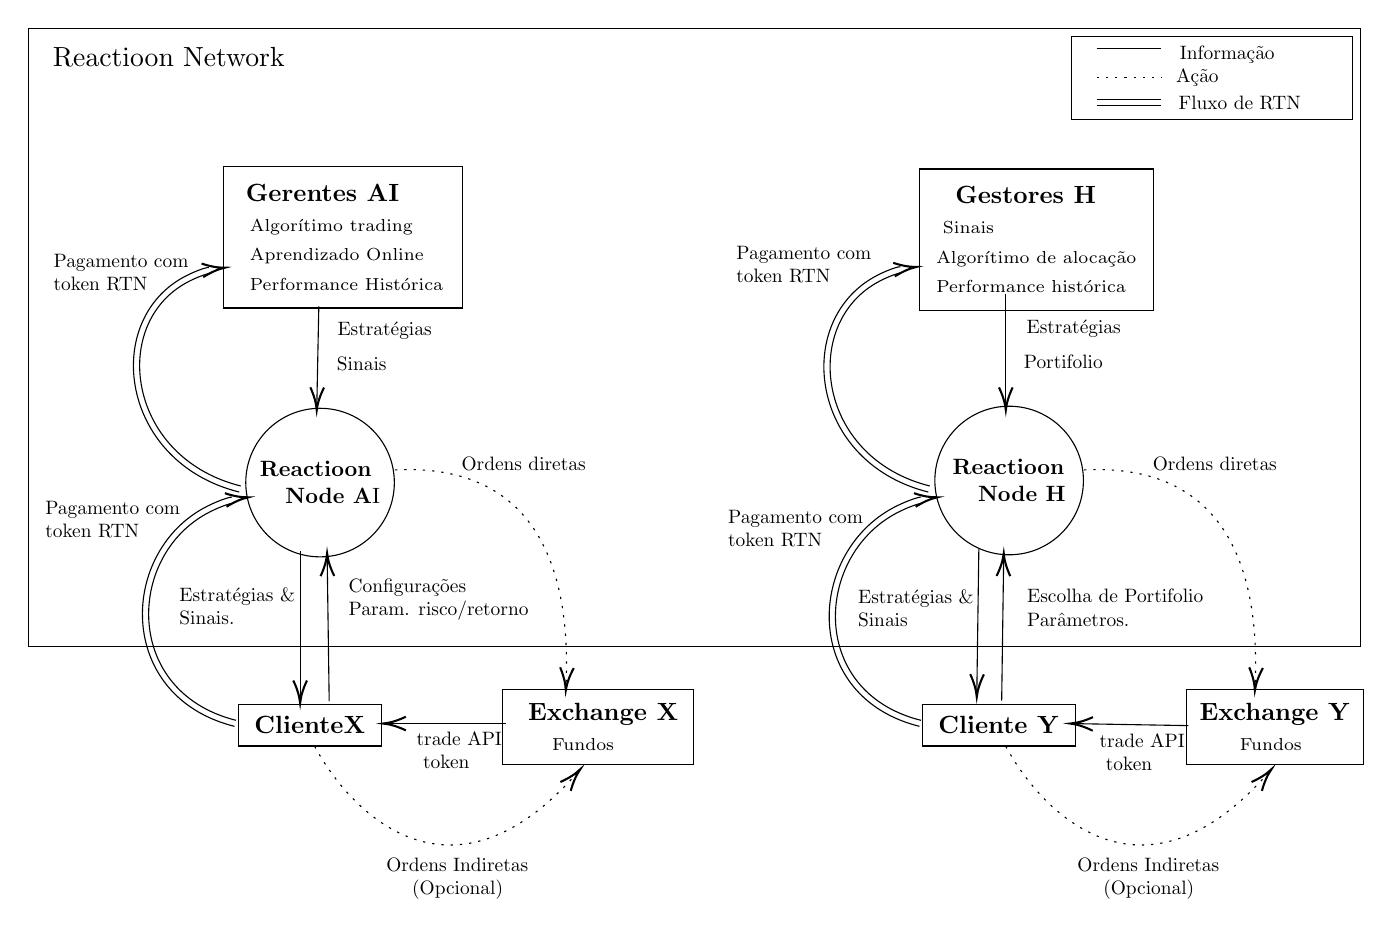
\begin{tikzpicture}[x=0.75pt,y=0.75pt,yscale=-1,xscale=1]
%uncomment if require: \path (0,464.1999969482422); %set diagram left start at 0, and has height of 464.1999969482422

%Shape: Rectangle [id:dp839607811925092] 
\draw   (16.3,16.2) -- (658.3,16.2) -- (658.3,314.2) -- (16.3,314.2) -- cycle ;
%Straight Lines [id:da3953078356379509] 
\draw    (156.3,150.2) -- (155.34,198.2) ;
\draw [shift={(155.3,200.2)}, rotate = 271.15] [color={rgb, 255:red, 0; green, 0; blue, 0 }  ][line width=0.75]    (10.93,-3.29) .. controls (6.95,-1.4) and (3.31,-0.3) .. (0,0) .. controls (3.31,0.3) and (6.95,1.4) .. (10.93,3.29)   ;

%Straight Lines [id:da5714023605084257] 
\draw    (246.3,351.2) -- (189.3,351.2) ;
\draw [shift={(187.3,351.2)}, rotate = 360] [color={rgb, 255:red, 0; green, 0; blue, 0 }  ][line width=0.75]    (10.93,-3.29) .. controls (6.95,-1.4) and (3.31,-0.3) .. (0,0) .. controls (3.31,0.3) and (6.95,1.4) .. (10.93,3.29)   ;

%Straight Lines [id:da41026468235715097] 
\draw    (161.3,340.4) -- (160.33,271.2) ;
\draw [shift={(160.3,269.2)}, rotate = 449.2] [color={rgb, 255:red, 0; green, 0; blue, 0 }  ][line width=0.75]    (10.93,-3.29) .. controls (6.95,-1.4) and (3.31,-0.3) .. (0,0) .. controls (3.31,0.3) and (6.95,1.4) .. (10.93,3.29)   ;

%Curve Lines [id:da9188372161085148] 
\draw  [dash pattern={on 0.84pt off 2.51pt}]  (193,229) .. controls (247.03,226.21) and (278.98,257.88) .. (275.36,334.05) ;
\draw [shift={(275.3,335.2)}, rotate = 272.97] [color={rgb, 255:red, 0; green, 0; blue, 0 }  ][line width=0.75]    (10.93,-3.29) .. controls (6.95,-1.4) and (3.31,-0.3) .. (0,0) .. controls (3.31,0.3) and (6.95,1.4) .. (10.93,3.29)   ;

%Curve Lines [id:da6611499345431215] 
\draw    (115.68,352.55) .. controls (92.15,346.66) and (78.57,331.56) .. (73.55,314.31) .. controls (72.05,309.15) and (71.32,303.8) .. (71.32,298.44) .. controls (71.32,298.19) and (71.32,297.93) .. (71.32,297.68) .. controls (71.58,277.85) and (81.85,258.04) .. (100.37,247.66) .. controls (106.22,244.39) and (112.89,242.05) .. (114.47,242.1)(116.41,349.64) .. controls (94.14,344.07) and (81.19,329.83) .. (76.43,313.47) .. controls (75.01,308.58) and (74.32,303.52) .. (74.32,298.44) .. controls (74.32,298.2) and (74.32,297.96) .. (74.32,297.72) .. controls (74.56,278.93) and (84.27,260.12) .. (101.84,250.28) .. controls (107.38,247.17) and (113.71,244.96) .. (114.91,245.09) ;
\draw [shift={(122.3,242.2)}, rotate = 533.23] [color={rgb, 255:red, 0; green, 0; blue, 0 }  ][line width=0.75]    (10.93,-3.29) .. controls (6.95,-1.4) and (3.31,-0.3) .. (0,0) .. controls (3.31,0.3) and (6.95,1.4) .. (10.93,3.29)   ;

%Curve Lines [id:da6558944188118099] 
\draw    (117.94,239.66) .. controls (91.22,232.98) and (75.05,214.75) .. (69.33,195.07) .. controls (68.48,192.12) and (67.85,189.14) .. (67.47,186.16) .. controls (67.14,183.68) and (66.98,181.21) .. (66.98,178.76) .. controls (66.98,161.73) and (74.72,145.63) .. (90.09,136.73) .. controls (95.48,133.61) and (101.81,131.38) .. (103.3,131.45)(118.66,236.74) .. controls (93.17,230.37) and (77.68,213.04) .. (72.22,194.23) .. controls (71.4,191.43) and (70.81,188.6) .. (70.44,185.77) .. controls (70.14,183.43) and (69.98,181.08) .. (69.98,178.76) .. controls (69.98,162.8) and (77.17,147.68) .. (91.6,139.33) .. controls (96.68,136.39) and (102.66,134.28) .. (103.68,134.45) ;
\draw [shift={(111.06,131.56)}, rotate = 533.23] [color={rgb, 255:red, 0; green, 0; blue, 0 }  ][line width=0.75]    (10.93,-3.29) .. controls (6.95,-1.4) and (3.31,-0.3) .. (0,0) .. controls (3.31,0.3) and (6.95,1.4) .. (10.93,3.29)   ;

%Curve Lines [id:da7197337789763143] 
\draw  [dash pattern={on 0.84pt off 2.51pt}]  (154.3,362.2) .. controls (173.2,397.02) and (221.81,442.74) .. (281.4,374.24) ;
\draw [shift={(282.3,373.2)}, rotate = 490.6] [color={rgb, 255:red, 0; green, 0; blue, 0 }  ][line width=0.75]    (10.93,-3.29) .. controls (6.95,-1.4) and (3.31,-0.3) .. (0,0) .. controls (3.31,0.3) and (6.95,1.4) .. (10.93,3.29)   ;

%Straight Lines [id:da7501707624311069] 
\draw    (487.3,144.2) -- (487.3,198.2) ;
\draw [shift={(487.3,200.2)}, rotate = 270] [color={rgb, 255:red, 0; green, 0; blue, 0 }  ][line width=0.75]    (10.93,-3.29) .. controls (6.95,-1.4) and (3.31,-0.3) .. (0,0) .. controls (3.31,0.3) and (6.95,1.4) .. (10.93,3.29)   ;

%Straight Lines [id:da11297405436688912] 
\draw    (575.3,352.2) -- (520.3,351.24) ;
\draw [shift={(518.3,351.2)}, rotate = 361.01] [color={rgb, 255:red, 0; green, 0; blue, 0 }  ][line width=0.75]    (10.93,-3.29) .. controls (6.95,-1.4) and (3.31,-0.3) .. (0,0) .. controls (3.31,0.3) and (6.95,1.4) .. (10.93,3.29)   ;

%Straight Lines [id:da9530469398494208] 
\draw    (485.3,340.2) -- (486.27,271.2) ;
\draw [shift={(486.3,269.2)}, rotate = 450.81] [color={rgb, 255:red, 0; green, 0; blue, 0 }  ][line width=0.75]    (10.93,-3.29) .. controls (6.95,-1.4) and (3.31,-0.3) .. (0,0) .. controls (3.31,0.3) and (6.95,1.4) .. (10.93,3.29)   ;

%Curve Lines [id:da6669727888364709] 
\draw  [dash pattern={on 0.84pt off 2.51pt}]  (525,229) .. controls (579.03,226.21) and (610.98,257.88) .. (607.36,334.05) ;
\draw [shift={(607.3,335.2)}, rotate = 272.97] [color={rgb, 255:red, 0; green, 0; blue, 0 }  ][line width=0.75]    (10.93,-3.29) .. controls (6.95,-1.4) and (3.31,-0.3) .. (0,0) .. controls (3.31,0.3) and (6.95,1.4) .. (10.93,3.29)   ;

%Curve Lines [id:da6929077991045711] 
\draw    (445.68,352.55) .. controls (422.54,346.76) and (409.27,332.05) .. (404.37,315.16) .. controls (402.91,310.12) and (402.2,304.87) .. (402.2,299.6) .. controls (402.2,298.95) and (402.21,298.3) .. (402.23,297.65) .. controls (402.9,277.57) and (413.86,257.51) .. (433.02,247.25) .. controls (438.74,244.19) and (445.19,242) .. (446.5,242.09)(446.41,349.64) .. controls (424.53,344.17) and (411.89,330.33) .. (407.26,314.33) .. controls (405.87,309.55) and (405.2,304.59) .. (405.2,299.6) .. controls (405.2,298.98) and (405.21,298.36) .. (405.23,297.75) .. controls (405.86,278.7) and (416.25,259.64) .. (434.43,249.9) .. controls (439.87,246.99) and (445.99,244.92) .. (446.94,245.08) ;
\draw [shift={(454.3,242.2)}, rotate = 533.23] [color={rgb, 255:red, 0; green, 0; blue, 0 }  ][line width=0.75]    (10.93,-3.29) .. controls (6.95,-1.4) and (3.31,-0.3) .. (0,0) .. controls (3.31,0.3) and (6.95,1.4) .. (10.93,3.29)   ;

%Curve Lines [id:da46112590181388846] 
\draw    (449.94,239.66) .. controls (423.51,233.05) and (407.61,215.09) .. (401.97,195.59) .. controls (401.05,192.4) and (400.4,189.18) .. (400.03,185.95) .. controls (399.77,183.73) and (399.64,181.5) .. (399.64,179.29) .. controls (399.64,162) and (407.53,145.57) .. (423.1,136.49) .. controls (428.56,133.31) and (434.97,131.03) .. (436.48,131.11)(450.66,236.74) .. controls (425.47,230.45) and (410.24,213.37) .. (404.85,194.75) .. controls (403.98,191.73) and (403.36,188.67) .. (403.01,185.61) .. controls (402.76,183.5) and (402.64,181.39) .. (402.64,179.29) .. controls (402.64,163.07) and (409.98,147.61) .. (424.62,139.09) .. controls (429.77,136.08) and (435.82,133.94) .. (436.95,134.08) ;
\draw [shift={(444.3,131.2)}, rotate = 533.23] [color={rgb, 255:red, 0; green, 0; blue, 0 }  ][line width=0.75]    (10.93,-3.29) .. controls (6.95,-1.4) and (3.31,-0.3) .. (0,0) .. controls (3.31,0.3) and (6.95,1.4) .. (10.93,3.29)   ;

%Curve Lines [id:da8354818907327548] 
\draw  [dash pattern={on 0.84pt off 2.51pt}]  (487.3,362.2) .. controls (506.2,397.02) and (554.81,442.74) .. (614.4,374.24) ;
\draw [shift={(615.3,373.2)}, rotate = 490.6] [color={rgb, 255:red, 0; green, 0; blue, 0 }  ][line width=0.75]    (10.93,-3.29) .. controls (6.95,-1.4) and (3.31,-0.3) .. (0,0) .. controls (3.31,0.3) and (6.95,1.4) .. (10.93,3.29)   ;

%Straight Lines [id:da8770926699692774] 
\draw    (147.3,268.2) -- (147.3,339.4) ;
\draw [shift={(147.3,341.4)}, rotate = 270] [color={rgb, 255:red, 0; green, 0; blue, 0 }  ][line width=0.75]    (10.93,-3.29) .. controls (6.95,-1.4) and (3.31,-0.3) .. (0,0) .. controls (3.31,0.3) and (6.95,1.4) .. (10.93,3.29)   ;

%Straight Lines [id:da36937072037759555] 
\draw    (474.3,267.2) -- (473.33,336.4) ;
\draw [shift={(473.3,338.4)}, rotate = 270.8] [color={rgb, 255:red, 0; green, 0; blue, 0 }  ][line width=0.75]    (10.93,-3.29) .. controls (6.95,-1.4) and (3.31,-0.3) .. (0,0) .. controls (3.31,0.3) and (6.95,1.4) .. (10.93,3.29)   ;

%Shape: Rectangle [id:dp03825033305531944] 
\draw   (518.9,20) -- (654.3,20) -- (654.3,60) -- (518.9,60) -- cycle ;
%Straight Lines [id:da5606203321141707] 
\draw    (531,26) -- (562.3,26) ;


%Straight Lines [id:da21375108102279738] 
\draw  [dash pattern={on 0.84pt off 2.51pt}]  (531,40) -- (562.3,40) ;


%Straight Lines [id:da15988012489637837] 
\draw    (531,50.5) -- (562.3,50.5)(531,53.5) -- (562.3,53.5) ;



% Text Node
\draw    (245,335) -- (337,335) -- (337,371) -- (245,371) -- cycle  ;
\draw (291,353) node [scale=0.9] [align=left] {\textbf{ Exchange X }\\{\scriptsize  \ \ \ \ \ Fundos}};
% Text Node
\draw    (117.5,342) -- (186.5,342) -- (186.5,362) -- (117.5,362) -- cycle  ;
\draw (152,352) node [scale=0.9] [align=left] {\textbf{ ClienteX }};
% Text Node
\draw    (110.5,83) -- (225.5,83) -- (225.5,151) -- (110.5,151) -- cycle  ;
\draw (168,117) node [scale=0.9] [align=left] {\textbf{ Gerentes AI}\\{\scriptsize  \ \ Algorítimo trading}\\{\scriptsize  \ \ Aprendizado Online \ }\\{\scriptsize  \ \ Performance Histórica \ }};
% Text Node
\draw    (156.9, 235.1) circle [x radius= 35.79, y radius= 35.79]   ;
\draw (156.9,235.1) node [scale=0.8] [align=left] {\textbf{Reactioon}\\\textbf{ \ \ Node A}I};
% Text Node
\draw (84,30) node  [align=left] {Reactioon Network};
% Text Node
\draw (224,364) node [scale=0.7] [align=left] {trade API \\ \ token};
% Text Node
\draw (188,162) node [scale=0.7] [align=left] {Estratégias};
% Text Node
\draw (177,178) node [scale=0.7] [align=left] {Sinais};
% Text Node
\draw (214,296) node [scale=0.7] [align=left] {Configurações\\Param. risco/retorno\\};
% Text Node
\draw (61,134) node [scale=0.7] [align=left] {Pagamento com\\ token RTN};
% Text Node
\draw (255,226) node [scale=0.7] [align=left] {Ordens diretas};
% Text Node
\draw (223,426) node [scale=0.7] [align=left] {Ordens Indiretas\\ \ \ \ \ (Opcional)};
% Text Node
\draw    (574.5,335) -- (659.5,335) -- (659.5,371) -- (574.5,371) -- cycle  ;
\draw (617,353) node [scale=0.9] [align=left] {\textbf{Exchange Y}\\{\scriptsize  \ \ \ \ \ \ Fundos}};
% Text Node
\draw    (447,342) -- (521,342) -- (521,362) -- (447,362) -- cycle  ;
\draw (484,352) node [scale=0.9] [align=left] {\textbf{ Cliente Y }};
% Text Node
\draw    (445.5,84) -- (558.5,84) -- (558.5,152) -- (445.5,152) -- cycle  ;
\draw (502,118) node [scale=0.9] [align=left] {\textbf{ \ Gestores H}\\{\scriptsize  \ Sinais}\\ {\scriptsize Algorítimo de alocação \ }\\{\scriptsize  Performance histórica }};
% Text Node
\draw    (488.9, 234.1) circle [x radius= 35.79, y radius= 35.79]   ;
\draw (488.9,234.1) node [scale=0.8] [align=left] {\textbf{Reactioon}\\\textbf{ \ \ Node H}};
% Text Node
\draw (540,301) node [scale=0.7] [align=left] {Escolha de Portifolio\\Parâmetros.\\};
% Text Node
\draw (588,226) node [scale=0.7] [align=left] {Ordens diretas};
% Text Node
\draw (117,306) node [scale=0.7] [align=left] {Estratégias \&\\Sinais.\\\\};
% Text Node
\draw (444,307) node [scale=0.7] [align=left] {Estratégias \&\\Sinais\\\\};
% Text Node
\draw (579.6,40) node [scale=0.7] [align=left] {Ação};
% Text Node
\draw (594,29) node [scale=0.7] [align=left] {Informação};
% Text Node
\draw (600,52) node [scale=0.7] [align=left] {Fluxo de RTN};
% Text Node
\draw (553,365) node [scale=0.7] [align=left] {trade API \\ \ token};
% Text Node
\draw (390,130) node [scale=0.7] [align=left] {Pagamento com\\ token RTN};
% Text Node
\draw (520,161) node [scale=0.7] [align=left] {Estratégias};
% Text Node
\draw (515,177) node [scale=0.7] [align=left] {Portifolio};
% Text Node
\draw (57,253) node [scale=0.7] [align=left] {Pagamento com\\ token RTN};
% Text Node
\draw (386,257) node [scale=0.7] [align=left] {Pagamento com\\ token RTN};
% Text Node
\draw (556,426) node [scale=0.7] [align=left] {Ordens Indiretas\\ \ \ \ \ (Opcional)};


\end{tikzpicture}
}
\caption{Reactioon network}
\end{figure}

Em ambos os tipos de contrato os usuários podem optar por não fornecer um token API, nesse caso, porém, deverão realizar os trades e alocações de recursos manualmente baseados em sinais fornecidos pelos nós do Reactioon. Nessa opção o usuário pagará por cada sinal adquirido individualmente. 

\section{Roadmap}
\subsection{Development steps}
Nesta seção apresentamos o Roadmap do projeto Reactioon, descrevemos cada etapa do desenvolvimento e nossos principais objetivos. A figura 2 ilustra todas as etapas planejadas para o projeto.

STEP O refere-se à Oferta Inicial de Moedas (ICO). Durante essa etapa, os tokens RTN serão emitidos para investidores alinhados com nossas ideias e interessados em nosso projeto. Nós classificamos os investidores em 3 tipos diferentes:
\begin{itemize}
    \item Level-0 refere-se aos investidores interessados apenas em comprar os tokens RTN para revenda futura, ou seja, aqueles que adotam a estratégia de HOLD. 
    \item Level-1 refere-se a investidores interessados em aumentar seu capital através da utilização dos serviços de gerenciamento da plataforma (trading bot e gerenciamento). Esses investidores são também chamados de clientes de ativos, pois são aqueles cujos ativos são gerenciados. 
    
    \item Level-3 refere-se a investidores que planejam comprar e operar seus próprios nós, seja como gerente de um nó-AI ou como gestor de um nó-H.
\end{itemize}

STEP 1 refere-se a de prova de conceito do projeto. Esta etapa foi planejada para ser realizada em paralelo com o ICO do projeto e consiste na disponibilização do serviço de trading bots (nós-AI) para os primeiros usuários do projeto. O objetivo é endossar a confiança no projeto e aumentar a exposição dos serviços oferecidos.

\begin{figure}[H]
    \centering
    \makebox[\textwidth]{


\tikzset{every picture/.style={line width=0.75pt}} %set default line width to 0.75pt        

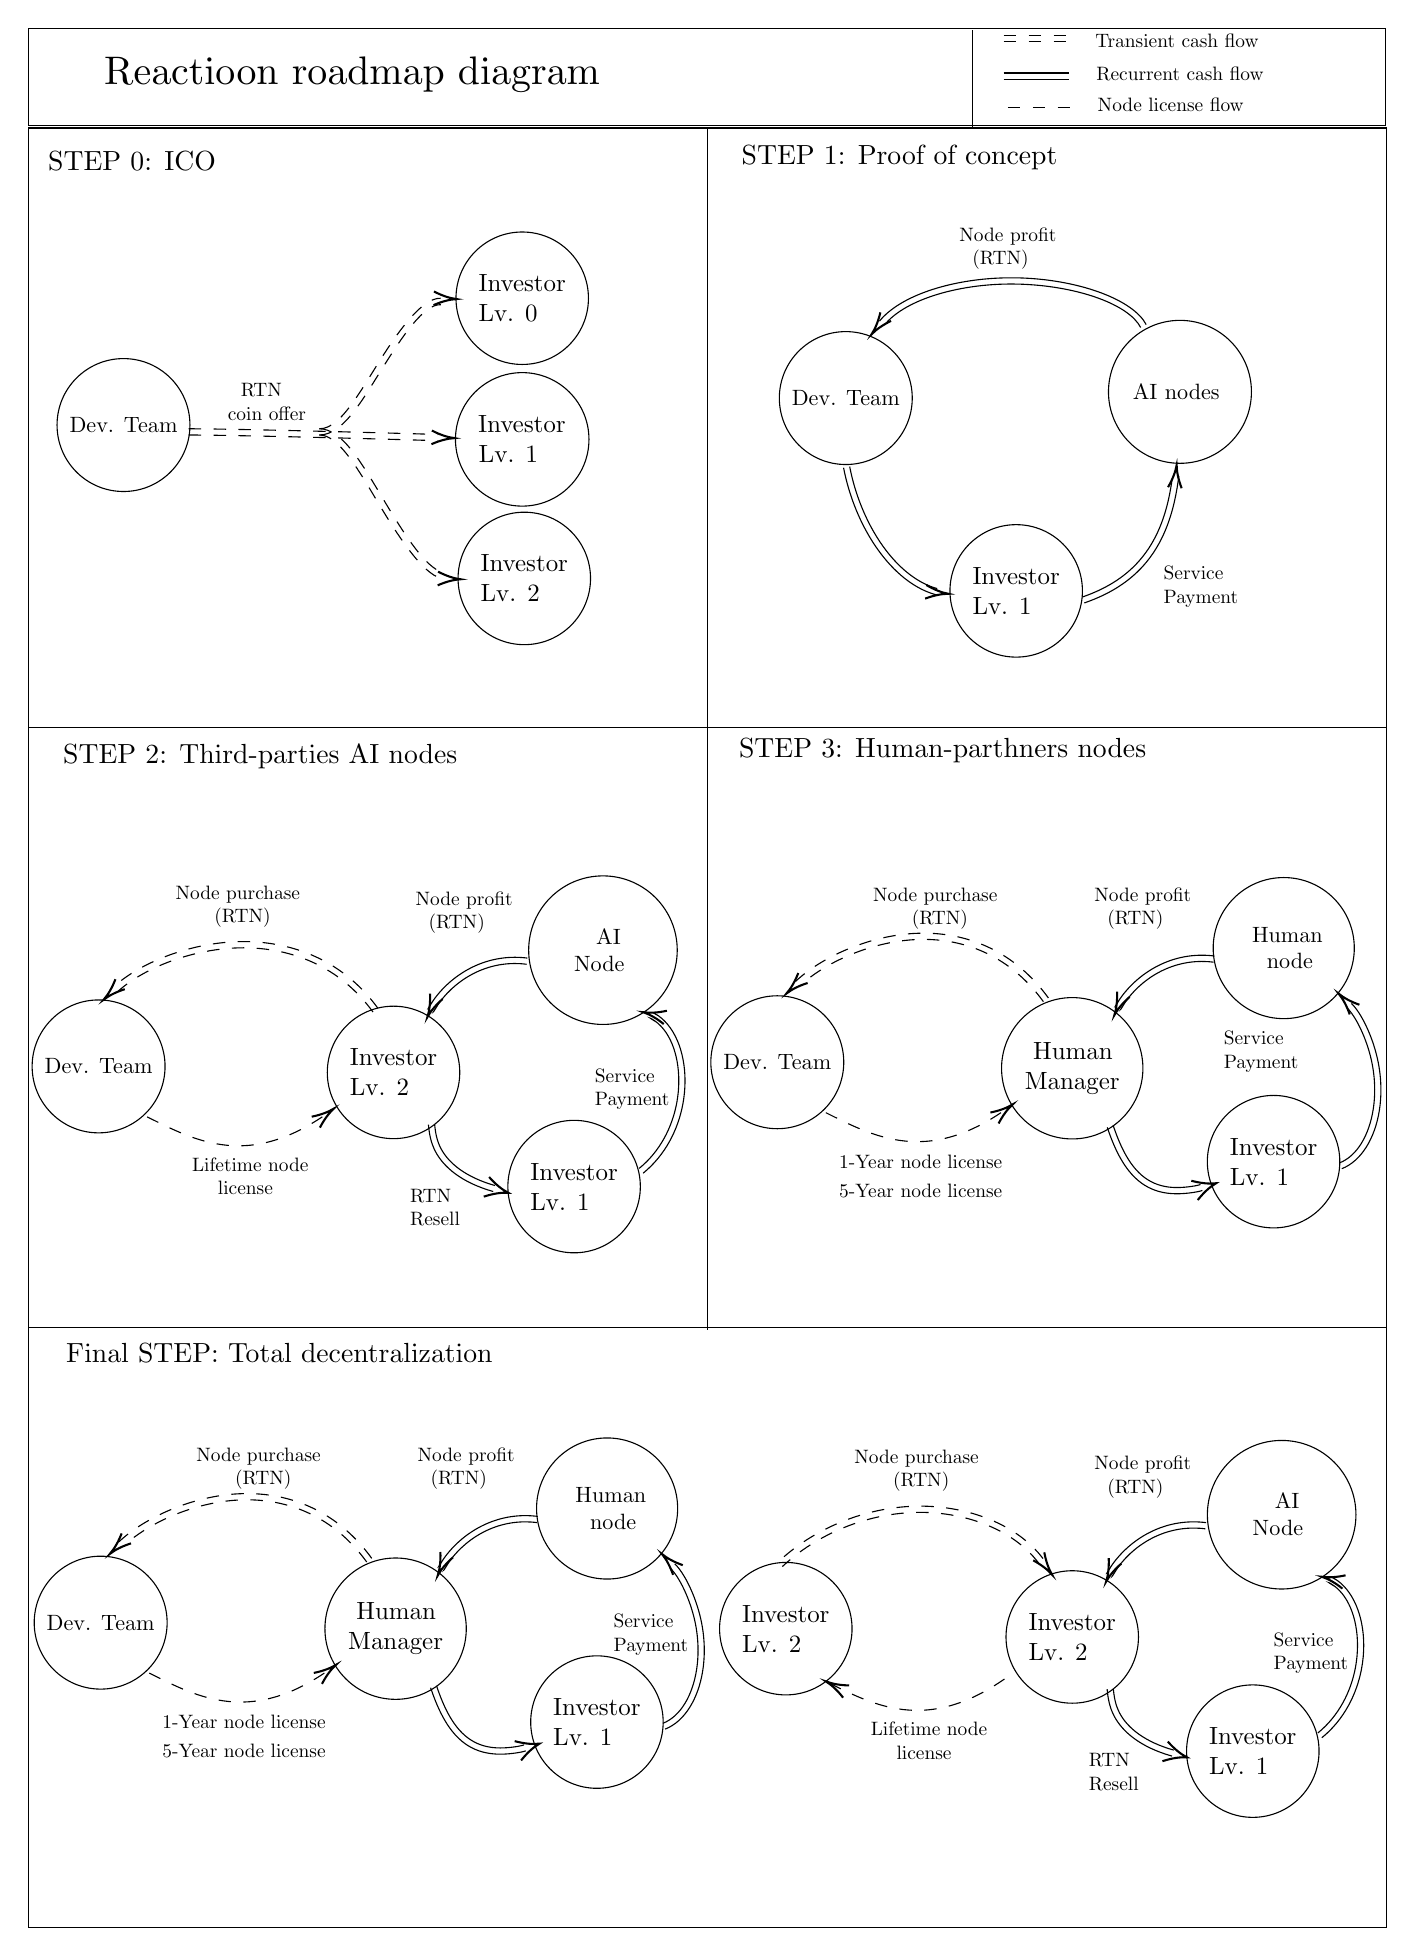
\begin{tikzpicture}[x=0.75pt,y=0.75pt,yscale=-1,xscale=1]
%uncomment if require: \path (0,979.6000061035156); %set diagram left start at 0, and has height of 979.6000061035156

%Curve Lines [id:da05976634933651925] 
\draw    (396.77,250.11) .. controls (401.92,276.72) and (417.5,301.22) .. (436.51,308.13) .. controls (438.57,308.87) and (440.67,309.41) .. (436.98,308.29)(393.83,250.69) .. controls (399.21,278.49) and (415.72,303.77) .. (435.49,310.95) .. controls (437.74,311.76) and (440.04,312.35) .. (436.54,311.31) ;
\draw [shift={(444.3,311.4)}, rotate = 184.97] [color={rgb, 255:red, 0; green, 0; blue, 0 }  ][line width=0.75]    (10.93,-3.29) .. controls (6.95,-1.4) and (3.31,-0.3) .. (0,0) .. controls (3.31,0.3) and (6.95,1.4) .. (10.93,3.29)   ;

%Curve Lines [id:da6305771665750117] 
\draw    (508.81,312.98) .. controls (530.84,305.36) and (545.51,291.1) .. (550.94,263.26) .. controls (551.69,259.42) and (552.27,255.33) .. (551.99,256.88)(509.79,315.82) .. controls (532.83,307.84) and (548.21,292.97) .. (553.89,263.83) .. controls (554.66,259.9) and (555.24,255.71) .. (554.98,257.17) ;
\draw [shift={(554.3,249.4)}, rotate = 454.51] [color={rgb, 255:red, 0; green, 0; blue, 0 }  ][line width=0.75]    (10.93,-3.29) .. controls (6.95,-1.4) and (3.31,-0.3) .. (0,0) .. controls (3.31,0.3) and (6.95,1.4) .. (10.93,3.29)   ;

%Curve Lines [id:da2780992376736433] 
\draw    (536.97,183.09) .. controls (531.13,171.91) and (506.97,163.46) .. (480.65,162.29) .. controls (478.64,162.2) and (476.6,162.16) .. (474.57,162.16) .. controls (472.28,162.16) and (469.98,162.21) .. (467.68,162.33) .. controls (445.29,163.49) and (422.84,170.39) .. (413.48,181.92)(539.63,181.71) .. controls (533.53,170.01) and (508.64,160.53) .. (480.78,159.29) .. controls (478.72,159.2) and (476.65,159.16) .. (474.57,159.16) .. controls (472.23,159.16) and (469.88,159.22) .. (467.53,159.34) .. controls (444.26,160.54) and (421.05,167.87) .. (411.11,180.04) ;
\draw [shift={(407.3,186.4)}, rotate = 308.65999999999997] [color={rgb, 255:red, 0; green, 0; blue, 0 }  ][line width=0.75]    (10.93,-3.29) .. controls (6.95,-1.4) and (3.31,-0.3) .. (0,0) .. controls (3.31,0.3) and (6.95,1.4) .. (10.93,3.29)   ;

%Curve Lines [id:da09682931505407599] 
\draw    (295.35,588.24) .. controls (305.49,579.98) and (311.3,568.29) .. (313.47,556.61) .. controls (314.12,553.06) and (314.44,549.5) .. (314.44,546.05) .. controls (314.44,533.02) and (309.94,521.23) .. (301.62,516.34) .. controls (300.63,515.76) and (299.6,515.28) .. (303.74,517.8)(297.25,590.56) .. controls (307.96,581.84) and (314.13,569.5) .. (316.42,557.15) .. controls (317.11,553.42) and (317.44,549.68) .. (317.44,546.05) .. controls (317.44,531.72) and (312.19,519.07) .. (303.14,513.75) .. controls (301.98,513.07) and (300.76,512.5) .. (304.78,514.82) ;
\draw [shift={(297.3,513)}, rotate = 373.21000000000004] [color={rgb, 255:red, 0; green, 0; blue, 0 }  ][line width=0.75]    (10.93,-3.29) .. controls (6.95,-1.4) and (3.31,-0.3) .. (0,0) .. controls (3.31,0.3) and (6.95,1.4) .. (10.93,3.29)   ;

%Straight Lines [id:da7893540143315829] 
\draw    (328.22,87) -- (328.22,666.2) ;


%Curve Lines [id:da1024768683684969] 
\draw    (225.02,599.37) .. controls (209.68,595.06) and (201.11,587.53) .. (197.2,580.12) .. controls (194.86,575.68) and (194.19,571.25) .. (193.81,567.14)(225.91,596.51) .. controls (211.81,592.55) and (203.54,585.7) .. (199.86,578.72) .. controls (197.72,574.66) and (197.14,570.61) .. (196.79,566.86) ;

\draw [shift={(232.3,600)}, rotate = 195.26] [color={rgb, 255:red, 0; green, 0; blue, 0 }  ][line width=0.75]    (10.93,-4.9) .. controls (6.95,-2.3) and (3.31,-0.67) .. (0,0) .. controls (3.31,0.67) and (6.95,2.3) .. (10.93,4.9)   ;
%Curve Lines [id:da669725253916299] 
\draw  [dash pattern={on 4.5pt off 4.5pt}]  (167.09,512.88) .. controls (151.26,491.1) and (128.15,481.96) .. (104.77,481.96) .. controls (103.86,481.96) and (102.94,481.98) .. (102.02,482) .. controls (78.89,482.71) and (55.75,492.2) .. (43.67,503.46)(169.51,511.12) .. controls (153.07,488.49) and (129.07,478.96) .. (104.77,478.96) .. controls (103.83,478.96) and (102.88,478.98) .. (101.93,479) .. controls (78.08,479.73) and (54.24,489.52) .. (41.78,501.13) ;
\draw [shift={(37.3,507)}, rotate = 316.74] [color={rgb, 255:red, 0; green, 0; blue, 0 }  ][line width=0.75]    (10.93,-3.29) .. controls (6.95,-1.4) and (3.31,-0.3) .. (0,0) .. controls (3.31,0.3) and (6.95,1.4) .. (10.93,3.29)   ;

%Curve Lines [id:da8285498578095596] 
\draw    (195.99,507.55) .. controls (193.21,512.09) and (193.61,511.35) .. (194.04,510.61) .. controls (201.02,498.57) and (215.98,486.53) .. (235.47,486.53) .. controls (237.43,486.53) and (239.44,486.66) .. (241.49,486.91)(198.71,508.9) .. controls (195.87,513.49) and (196.24,512.8) .. (196.63,512.12) .. controls (203.18,500.83) and (217.2,489.53) .. (235.47,489.53) .. controls (237.31,489.53) and (239.19,489.65) .. (241.11,489.89) ;

\draw [shift={(193.3,515.4)}, rotate = 293.2] [color={rgb, 255:red, 0; green, 0; blue, 0 }  ][line width=0.75]    (10.93,-3.29) .. controls (6.95,-1.4) and (3.31,-0.3) .. (0,0) .. controls (3.31,0.3) and (6.95,1.4) .. (10.93,3.29)   ;
%Curve Lines [id:da692172908683615] 
\draw  [dash pattern={on 4.5pt off 4.5pt}]  (58.3,563.4) .. controls (82.06,575.28) and (107.78,589.12) .. (147.1,560.29) ;
\draw [shift={(148.3,559.4)}, rotate = 503.13] [color={rgb, 255:red, 0; green, 0; blue, 0 }  ][line width=0.75]    (10.93,-3.29) .. controls (6.95,-1.4) and (3.31,-0.3) .. (0,0) .. controls (3.31,0.3) and (6.95,1.4) .. (10.93,3.29)   ;

%Shape: Rectangle [id:dp40281470565409405] 
\draw   (1,87) -- (655.3,87) -- (655.3,376) -- (1,376) -- cycle ;
%Shape: Rectangle [id:dp9634875424623359] 
\draw   (1,376) -- (655.3,376) -- (655.3,665) -- (1,665) -- cycle ;
%Curve Lines [id:da5815941848800827] 
\draw  [dash pattern={on 4.5pt off 4.5pt}]  (78.3,231.9) .. controls (89.72,231.9) and (117.71,232.49) .. (145.7,233.19) .. controls (152.02,233.35) and (158.35,233.51) .. (164.49,233.68) .. controls (180.12,234.1) and (194.51,234.51) .. (198.52,234.65)(78.3,234.9) .. controls (89.71,234.9) and (117.67,235.49) .. (145.62,236.19) .. controls (151.95,236.35) and (158.27,236.51) .. (164.41,236.68) .. controls (180.04,237.09) and (194.42,237.51) .. (198.43,237.65) ;
\draw [shift={(206.3,236.4)}, rotate = 181.91] [color={rgb, 255:red, 0; green, 0; blue, 0 }  ][line width=0.75]    (10.93,-3.29) .. controls (6.95,-1.4) and (3.31,-0.3) .. (0,0) .. controls (3.31,0.3) and (6.95,1.4) .. (10.93,3.29)   ;

%Curve Lines [id:da08986855838242058] 
\draw  [dash pattern={on 4.5pt off 4.5pt}]  (141.3,231.9) .. controls (146.94,231.9) and (151.99,226.67) .. (157.11,219.65) .. controls (161.15,214.11) and (165.19,207.35) .. (169.42,200.6) .. controls (179.53,184.47) and (190.83,168.71) .. (199.7,169.02)(141.3,234.9) .. controls (147.66,234.9) and (153.63,229.52) .. (159.53,221.42) .. controls (163.61,215.83) and (167.69,209.01) .. (171.96,202.19) .. controls (181.42,187.11) and (191.75,171.66) .. (199.79,172.12) ;
\draw [shift={(207.3,169.4)}, rotate = 181.91] [color={rgb, 255:red, 0; green, 0; blue, 0 }  ][line width=0.75]    (10.93,-3.29) .. controls (6.95,-1.4) and (3.31,-0.3) .. (0,0) .. controls (3.31,0.3) and (6.95,1.4) .. (10.93,3.29)   ;

%Curve Lines [id:da39444446904774755] 
\draw  [dash pattern={on 4.5pt off 4.5pt}]  (141.3,231.9) .. controls (146.59,231.9) and (151.75,235.86) .. (156.86,242.28) .. controls (162.27,249.1) and (167.69,258.61) .. (173.44,268.13) .. controls (183.28,284.42) and (194,301.05) .. (202.12,301.21)(141.3,234.9) .. controls (145.89,234.9) and (150.17,238.69) .. (154.51,244.15) .. controls (159.85,250.88) and (165.2,260.28) .. (170.87,269.68) .. controls (181.31,286.98) and (192.94,303.94) .. (201.65,304.22) ;
\draw [shift={(209.3,304.4)}, rotate = 181.91] [color={rgb, 255:red, 0; green, 0; blue, 0 }  ][line width=0.75]    (10.93,-3.29) .. controls (6.95,-1.4) and (3.31,-0.3) .. (0,0) .. controls (3.31,0.3) and (6.95,1.4) .. (10.93,3.29)   ;

%Curve Lines [id:da22052512179005368] 
\draw    (632.75,585.6) .. controls (641.29,582.27) and (647.07,572.15) .. (649.01,559.76) .. controls (649.48,556.78) and (649.72,553.65) .. (649.72,550.45) .. controls (649.72,545.71) and (649.19,540.79) .. (648.08,535.88) .. controls (645.7,525.45) and (640.69,515.02) .. (636.26,510.75)(633.85,588.4) .. controls (643.17,584.75) and (649.83,573.92) .. (651.98,560.22) .. controls (652.47,557.09) and (652.72,553.81) .. (652.72,550.45) .. controls (652.72,545.49) and (652.17,540.35) .. (651,535.21) .. controls (648.52,524.29) and (643.26,513.37) .. (638.51,508.75) ;
\draw [shift={(632.3,504)}, rotate = 405] [color={rgb, 255:red, 0; green, 0; blue, 0 }  ][line width=0.75]    (10.93,-3.29) .. controls (6.95,-1.4) and (3.31,-0.3) .. (0,0) .. controls (3.31,0.3) and (6.95,1.4) .. (10.93,3.29)   ;

%Curve Lines [id:da6010390464009561] 
\draw    (566.7,598.86) .. controls (565.11,599.5) and (559.43,600.47) .. (554.43,600.47) .. controls (542.25,600.47) and (533.91,594.86) .. (527.58,583.95) .. controls (525.07,579.63) and (522.87,574.46) .. (520.88,568.47)(565.81,595.99) .. controls (564.56,596.53) and (559.18,597.47) .. (554.43,597.47) .. controls (543.39,597.47) and (535.9,592.3) .. (530.17,582.44) .. controls (527.75,578.28) and (525.65,573.3) .. (523.72,567.53) ;

\draw [shift={(573.3,595.4)}, rotate = 161.68] [color={rgb, 255:red, 0; green, 0; blue, 0 }  ][line width=0.75]    (10.93,-4.9) .. controls (6.95,-2.3) and (3.31,-0.67) .. (0,0) .. controls (3.31,0.67) and (6.95,2.3) .. (10.93,4.9)   ;
%Curve Lines [id:da4285918232372201] 
\draw  [dash pattern={on 4.5pt off 4.5pt}]  (490.09,507.88) .. controls (474.69,486.7) and (453.74,477.91) .. (432.42,477.91) .. controls (430.9,477.91) and (429.38,477.95) .. (427.86,478.04) .. controls (406.24,479.29) and (384.63,489.24) .. (372.86,500.25)(492.51,506.12) .. controls (476.47,484.05) and (454.63,474.91) .. (432.42,474.91) .. controls (430.84,474.91) and (429.27,474.96) .. (427.69,475.05) .. controls (405.4,476.33) and (383.11,486.56) .. (370.71,498.13) ;
\draw [shift={(366.3,504)}, rotate = 316.74] [color={rgb, 255:red, 0; green, 0; blue, 0 }  ][line width=0.75]    (10.93,-3.29) .. controls (6.95,-1.4) and (3.31,-0.3) .. (0,0) .. controls (3.31,0.3) and (6.95,1.4) .. (10.93,3.29)   ;

%Curve Lines [id:da5188301134475544] 
\draw    (526.99,506.55) .. controls (524.21,511.09) and (524.61,510.35) .. (525.04,509.61) .. controls (532.02,497.57) and (546.98,485.53) .. (566.47,485.53) .. controls (568.43,485.53) and (570.44,485.66) .. (572.49,485.91)(529.71,507.9) .. controls (526.87,512.49) and (527.24,511.8) .. (527.63,511.12) .. controls (534.18,499.83) and (548.2,488.53) .. (566.47,488.53) .. controls (568.31,488.53) and (570.19,488.65) .. (572.11,488.89) ;

\draw [shift={(524.3,514.4)}, rotate = 293.2] [color={rgb, 255:red, 0; green, 0; blue, 0 }  ][line width=0.75]    (10.93,-3.29) .. controls (6.95,-1.4) and (3.31,-0.3) .. (0,0) .. controls (3.31,0.3) and (6.95,1.4) .. (10.93,3.29)   ;
%Curve Lines [id:da6657104804294918] 
\draw  [dash pattern={on 4.5pt off 4.5pt}]  (385.3,561.4) .. controls (409.06,573.28) and (434.78,587.12) .. (474.1,558.29) ;
\draw [shift={(475.3,557.4)}, rotate = 503.13] [color={rgb, 255:red, 0; green, 0; blue, 0 }  ][line width=0.75]    (10.93,-3.29) .. controls (6.95,-1.4) and (3.31,-0.3) .. (0,0) .. controls (3.31,0.3) and (6.95,1.4) .. (10.93,3.29)   ;

%Shape: Rectangle [id:dp6670442393793834] 
\draw   (1,665) -- (655.3,665) -- (655.3,954) -- (1,954) -- cycle ;
%Curve Lines [id:da6777059505251721] 
\draw    (622.35,860.24) .. controls (632.49,851.98) and (638.3,840.29) .. (640.47,828.61) .. controls (641.12,825.06) and (641.44,821.5) .. (641.44,818.05) .. controls (641.44,805.02) and (636.94,793.23) .. (628.62,788.34) .. controls (627.63,787.76) and (626.6,787.28) .. (630.74,789.8)(624.25,862.56) .. controls (634.96,853.84) and (641.13,841.5) .. (643.42,829.15) .. controls (644.11,825.42) and (644.44,821.68) .. (644.44,818.05) .. controls (644.44,803.72) and (639.19,791.07) .. (630.14,785.75) .. controls (628.98,785.07) and (627.76,784.5) .. (631.78,786.82) ;
\draw [shift={(624.3,785)}, rotate = 373.21000000000004] [color={rgb, 255:red, 0; green, 0; blue, 0 }  ][line width=0.75]    (10.93,-3.29) .. controls (6.95,-1.4) and (3.31,-0.3) .. (0,0) .. controls (3.31,0.3) and (6.95,1.4) .. (10.93,3.29)   ;

%Curve Lines [id:da7795529337986824] 
\draw    (552.02,871.37) .. controls (536.68,867.06) and (528.11,859.53) .. (524.2,852.12) .. controls (521.86,847.68) and (521.19,843.25) .. (520.81,839.14)(552.91,868.51) .. controls (538.81,864.55) and (530.54,857.7) .. (526.86,850.72) .. controls (524.72,846.66) and (524.14,842.61) .. (523.79,838.86) ;

\draw [shift={(559.3,872)}, rotate = 195.26] [color={rgb, 255:red, 0; green, 0; blue, 0 }  ][line width=0.75]    (10.93,-4.9) .. controls (6.95,-2.3) and (3.31,-0.67) .. (0,0) .. controls (3.31,0.67) and (6.95,2.3) .. (10.93,4.9)   ;
%Curve Lines [id:da7053921066585791] 
\draw  [dash pattern={on 4.5pt off 4.5pt}]  (487.7,778.25) .. controls (475.84,762.55) and (453.43,753.96) .. (430.77,753.96) .. controls (429.86,753.96) and (428.94,753.98) .. (428.02,754) .. controls (404.41,754.72) and (380.8,764.59) .. (364.33,780.09)(489.92,776.23) .. controls (477.59,759.92) and (454.32,750.96) .. (430.77,750.96) .. controls (429.83,750.96) and (428.88,750.98) .. (427.93,751) .. controls (403.59,751.74) and (379.25,761.93) .. (362.27,777.91) ;

\draw [shift={(494.3,784)}, rotate = 233.99] [color={rgb, 255:red, 0; green, 0; blue, 0 }  ][line width=0.75]    (10.93,-3.29) .. controls (6.95,-1.4) and (3.31,-0.3) .. (0,0) .. controls (3.31,0.3) and (6.95,1.4) .. (10.93,3.29)   ;
%Curve Lines [id:da652710059709394] 
\draw    (522.99,779.55) .. controls (520.21,784.09) and (520.61,783.35) .. (521.04,782.61) .. controls (528.02,770.57) and (542.98,758.53) .. (562.47,758.53) .. controls (564.43,758.53) and (566.44,758.66) .. (568.49,758.91)(525.71,780.9) .. controls (522.87,785.49) and (523.24,784.8) .. (523.63,784.12) .. controls (530.18,772.83) and (544.2,761.53) .. (562.47,761.53) .. controls (564.31,761.53) and (566.19,761.65) .. (568.11,761.89) ;

\draw [shift={(520.3,787.4)}, rotate = 293.2] [color={rgb, 255:red, 0; green, 0; blue, 0 }  ][line width=0.75]    (10.93,-3.29) .. controls (6.95,-1.4) and (3.31,-0.3) .. (0,0) .. controls (3.31,0.3) and (6.95,1.4) .. (10.93,3.29)   ;
%Curve Lines [id:da6969687500387687] 
\draw  [dash pattern={on 4.5pt off 4.5pt}]  (387.1,836.3) .. controls (410.61,848.07) and (436.3,860.65) .. (475.3,831.4) ;

\draw [shift={(385.3,835.4)}, rotate = 26.57] [color={rgb, 255:red, 0; green, 0; blue, 0 }  ][line width=0.75]    (10.93,-3.29) .. controls (6.95,-1.4) and (3.31,-0.3) .. (0,0) .. controls (3.31,0.3) and (6.95,1.4) .. (10.93,3.29)   ;
%Curve Lines [id:da3295133955045202] 
\draw    (306.75,855.6) .. controls (315.29,852.27) and (321.07,842.15) .. (323.01,829.76) .. controls (323.48,826.78) and (323.72,823.65) .. (323.72,820.45) .. controls (323.72,815.71) and (323.19,810.79) .. (322.08,805.88) .. controls (319.7,795.45) and (314.69,785.02) .. (310.26,780.75)(307.85,858.4) .. controls (317.17,854.75) and (323.83,843.92) .. (325.98,830.22) .. controls (326.47,827.09) and (326.72,823.81) .. (326.72,820.45) .. controls (326.72,815.49) and (326.17,810.35) .. (325,805.21) .. controls (322.52,794.29) and (317.26,783.37) .. (312.51,778.75) ;
\draw [shift={(306.3,774)}, rotate = 405] [color={rgb, 255:red, 0; green, 0; blue, 0 }  ][line width=0.75]    (10.93,-3.29) .. controls (6.95,-1.4) and (3.31,-0.3) .. (0,0) .. controls (3.31,0.3) and (6.95,1.4) .. (10.93,3.29)   ;

%Curve Lines [id:da7666769359917143] 
\draw    (240.7,868.86) .. controls (239.11,869.5) and (233.43,870.47) .. (228.43,870.47) .. controls (216.25,870.47) and (207.91,864.86) .. (201.58,853.95) .. controls (199.07,849.63) and (196.87,844.46) .. (194.88,838.47)(239.81,865.99) .. controls (238.56,866.53) and (233.18,867.47) .. (228.43,867.47) .. controls (217.39,867.47) and (209.9,862.3) .. (204.17,852.44) .. controls (201.75,848.28) and (199.65,843.3) .. (197.72,837.53) ;

\draw [shift={(247.3,865.4)}, rotate = 161.68] [color={rgb, 255:red, 0; green, 0; blue, 0 }  ][line width=0.75]    (10.93,-4.9) .. controls (6.95,-2.3) and (3.31,-0.67) .. (0,0) .. controls (3.31,0.67) and (6.95,2.3) .. (10.93,4.9)   ;
%Curve Lines [id:da46762012302444633] 
\draw  [dash pattern={on 4.5pt off 4.5pt}]  (164.09,777.88) .. controls (148.69,756.7) and (127.74,747.91) .. (106.42,747.91) .. controls (104.9,747.91) and (103.38,747.95) .. (101.86,748.04) .. controls (80.24,749.29) and (58.63,759.24) .. (46.86,770.25)(166.51,776.12) .. controls (150.47,754.05) and (128.63,744.91) .. (106.42,744.91) .. controls (104.84,744.91) and (103.27,744.96) .. (101.69,745.05) .. controls (79.4,746.33) and (57.11,756.56) .. (44.71,768.13) ;
\draw [shift={(40.3,774)}, rotate = 316.74] [color={rgb, 255:red, 0; green, 0; blue, 0 }  ][line width=0.75]    (10.93,-3.29) .. controls (6.95,-1.4) and (3.31,-0.3) .. (0,0) .. controls (3.31,0.3) and (6.95,1.4) .. (10.93,3.29)   ;

%Curve Lines [id:da48374864838781084] 
\draw    (200.99,776.55) .. controls (198.21,781.09) and (198.61,780.35) .. (199.04,779.61) .. controls (206.02,767.57) and (220.98,755.53) .. (240.47,755.53) .. controls (242.43,755.53) and (244.44,755.66) .. (246.49,755.91)(203.71,777.9) .. controls (200.87,782.49) and (201.24,781.8) .. (201.63,781.12) .. controls (208.18,769.83) and (222.2,758.53) .. (240.47,758.53) .. controls (242.31,758.53) and (244.19,758.65) .. (246.11,758.89) ;

\draw [shift={(198.3,784.4)}, rotate = 293.2] [color={rgb, 255:red, 0; green, 0; blue, 0 }  ][line width=0.75]    (10.93,-3.29) .. controls (6.95,-1.4) and (3.31,-0.3) .. (0,0) .. controls (3.31,0.3) and (6.95,1.4) .. (10.93,3.29)   ;
%Curve Lines [id:da5692917843664225] 
\draw  [dash pattern={on 4.5pt off 4.5pt}]  (59.3,831.4) .. controls (83.06,843.28) and (108.78,857.12) .. (148.1,828.29) ;
\draw [shift={(149.3,827.4)}, rotate = 503.13] [color={rgb, 255:red, 0; green, 0; blue, 0 }  ][line width=0.75]    (10.93,-3.29) .. controls (6.95,-1.4) and (3.31,-0.3) .. (0,0) .. controls (3.31,0.3) and (6.95,1.4) .. (10.93,3.29)   ;

%Straight Lines [id:da04624544215982018] 
\draw  [dash pattern={on 4.5pt off 4.5pt}]  (471,42.5) -- (502.3,42.5)(471,45.5) -- (502.3,45.5) ;


%Straight Lines [id:da8337419241786759] 
\draw    (471,60.5) -- (502.3,60.5)(471,63.5) -- (502.3,63.5) ;


%Shape: Rectangle [id:dp8280881989403395] 
\draw   (1,39) -- (654.9,39) -- (654.9,85.8) -- (1,85.8) -- cycle ;
%Straight Lines [id:da6253908926711176] 
\draw    (455.9,40) -- (455.9,86.64) ;


%Straight Lines [id:da08377365797985514] 
\draw  [dash pattern={on 4.5pt off 4.5pt}]  (473,77) -- (504.3,77) ;



% Text Node
\draw    (477, 310) circle [x radius= 31.91, y radius= 31.91]   ;
\draw (477,310) node [scale=0.9] [align=left] {Investor\\Lv. 1};
% Text Node
\draw    (555.9, 214.1) circle [x radius= 34.44, y radius= 34.44]   ;
\draw (555.9,214.1) node [scale=0.8] [align=left] { \ AI nodes \ };
% Text Node
\draw    (394.9, 217.1) circle [x radius= 32.02, y radius= 32.02]   ;
\draw (394.9,217.1) node [scale=0.8] [align=left] {Dev. Team};
% Text Node
\draw    (177, 542) circle [x radius= 31.91, y radius= 31.91]   ;
\draw (177,542) node [scale=0.9] [align=left] {Investor\\ Lv. 2};
% Text Node
\draw    (277.9, 483.1) circle [x radius= 35.79, y radius= 35.79]   ;
\draw (277.9,483.1) node [scale=0.8] [align=left] { \ \ \ \ \ \ AI\\ \ \ \ Node \ \ \ \ };
% Text Node
\draw    (34.9, 539.1) circle [x radius= 32.02, y radius= 32.02]   ;
\draw (34.9,539.1) node [scale=0.8] [align=left] {Dev. Team};
% Text Node
\draw (292,550) node [scale=0.7] [align=left] {Service \\Payment};
% Text Node
\draw (423,101) node  [align=left] {STEP 1: Proof of concept };
% Text Node
\draw (115,390) node  [align=left] {STEP 2: Third-parties AI nodes };
% Text Node
\draw    (264, 597) circle [x radius= 31.91, y radius= 31.91]   ;
\draw (264,597) node [scale=0.9] [align=left] {Investor\\Lv. 1};
% Text Node
\draw (102,462) node [scale=0.7] [align=left] {Node purchase \\ \ \ \ \ \ \ (RTN)};
% Text Node
\draw (108,592) node [scale=0.7] [align=left] {Lifetime node\\ \ \ \ \ license};
% Text Node
\draw (211,465) node [scale=0.7] [align=left] {Node profit\\ \ \ (RTN)};
% Text Node
\draw    (46.9, 230.1) circle [x radius= 32.02, y radius= 32.02]   ;
\draw (46.9,230.1) node [scale=0.8] [align=left] {Dev. Team};
% Text Node
\draw (566,308) node [scale=0.7] [align=left] {Service \\Payment};
% Text Node
\draw (51,103) node  [align=left] {STEP 0: ICO};
% Text Node
\draw (116,219) node [scale=0.7] [align=left] { \ \ RTN \\ coin offer};
% Text Node
\draw (473,145) node [scale=0.7] [align=left] {Node profit\\ \ \ (RTN)};
% Text Node
\draw    (239, 169) circle [x radius= 31.91, y radius= 31.91]   ;
\draw (239,169) node [scale=0.9] [align=left] {Investor\\ Lv. 0};
% Text Node
\draw    (239, 237) circle [x radius= 32.16, y radius= 32.16]   ;
\draw (239,237) node [scale=0.9,xslant=-0.02] [align=left] {Investor\\ Lv. 1};
% Text Node
\draw    (240, 304) circle [x radius= 31.91, y radius= 31.91]   ;
\draw (240,304) node [scale=0.9] [align=left] {Investor\\ Lv. 2};
% Text Node
\draw    (504, 540) circle [x radius= 34.05, y radius= 34.05]   ;
\draw (504,540) node [scale=0.9] [align=left] { \ Human\\Manager};
% Text Node
\draw    (605.9, 482.1) circle [x radius= 33.99, y radius= 33.99]   ;
\draw (605.9,482.1) node [scale=0.8] [align=left] { \ \ Human \ \\ \ \ \ \ node};
% Text Node
\draw    (361.9, 537.1) circle [x radius= 32.02, y radius= 32.02]   ;
\draw (361.9,537.1) node [scale=0.8] [align=left] {Dev. Team};
% Text Node
\draw (595,532) node [scale=0.7] [align=left] {Service \\Payment};
% Text Node
\draw (446,387) node  [align=left] { STEP 3: Human-parthners nodes \ };
% Text Node
\draw    (601, 585) circle [x radius= 31.91, y radius= 31.91]   ;
\draw (601,585) node [scale=0.9] [align=left] {Investor\\Lv. 1};
% Text Node
\draw (431,585) node [scale=0.7] [align=left] {1-Year node license};
% Text Node
\draw (538,463) node [scale=0.7] [align=left] {Node profit\\ \ \ (RTN)};
% Text Node
\draw (197,607) node [scale=0.7] [align=left] {RTN\\Resell};
% Text Node
\draw (438,463) node [scale=0.7] [align=left] {Node purchase \\ \ \ \ \ \ \ (RTN)};
% Text Node
\draw (431,599) node [scale=0.7] [align=left] {5-Year node license};
% Text Node
\draw (122,677) node  [align=left] {Final STEP: Total decentralization};
% Text Node
\draw    (504, 814) circle [x radius= 31.91, y radius= 31.91]   ;
\draw (504,814) node [scale=0.9] [align=left] {Investor\\ Lv. 2};
% Text Node
\draw    (604.9, 755.1) circle [x radius= 35.79, y radius= 35.79]   ;
\draw (604.9,755.1) node [scale=0.8] [align=left] { \ \ \ \ \ \ AI\\ \ \ \ Node \ \ \ \ };
% Text Node
\draw (619,822) node [scale=0.7] [align=left] {Service \\Payment};
% Text Node
\draw    (591, 869) circle [x radius= 31.91, y radius= 31.91]   ;
\draw (591,869) node [scale=0.9] [align=left] {Investor\\Lv. 1};
% Text Node
\draw (429,734) node [scale=0.7] [align=left] {Node purchase \\ \ \ \ \ \ \ (RTN)};
% Text Node
\draw (435,864) node [scale=0.7] [align=left] {Lifetime node\\ \ \ \ \ license};
% Text Node
\draw (538,737) node [scale=0.7] [align=left] {Node profit\\ \ \ (RTN)};
% Text Node
\draw (524,879) node [scale=0.7] [align=left] {RTN\\Resell};
% Text Node
\draw    (366, 810) circle [x radius= 31.91, y radius= 31.91]   ;
\draw (366,810) node [scale=0.9] [align=left] {Investor\\ Lv. 2};
% Text Node
\draw    (178, 810) circle [x radius= 34.05, y radius= 34.05]   ;
\draw (178,810) node [scale=0.9] [align=left] { \ Human\\Manager};
% Text Node
\draw    (279.9, 752.1) circle [x radius= 33.99, y radius= 33.99]   ;
\draw (279.9,752.1) node [scale=0.8] [align=left] { \ \ Human \ \\ \ \ \ \ node};
% Text Node
\draw    (35.9, 807.1) circle [x radius= 32.02, y radius= 32.02]   ;
\draw (35.9,807.1) node [scale=0.8] [align=left] {Dev. Team};
% Text Node
\draw (301,813) node [scale=0.7] [align=left] {Service \\Payment};
% Text Node
\draw    (275, 855) circle [x radius= 31.91, y radius= 31.91]   ;
\draw (275,855) node [scale=0.9] [align=left] {Investor\\Lv. 1};
% Text Node
\draw (105,855) node [scale=0.7] [align=left] {1-Year node license};
% Text Node
\draw (212,733) node [scale=0.7] [align=left] {Node profit\\ \ \ (RTN)};
% Text Node
\draw (112,733) node [scale=0.7] [align=left] {Node purchase \\ \ \ \ \ \ \ (RTN)};
% Text Node
\draw (105,869) node [scale=0.7] [align=left] {5-Year node license};
% Text Node
\draw (556,45) node [scale=0.7] [align=left] {Transient cash flow };
% Text Node
\draw (553,76) node [scale=0.7] [align=left] {Node license flow };
% Text Node
\draw (559,61) node [scale=0.7] [align=left] {Recurrent cash flow \ };
% Text Node
\draw (157,61) node [scale=1.44] [align=left] {Reactioon roadmap diagram};


\end{tikzpicture}
}
\caption{Roadmap diagram}
\end{figure}
STEP 2 refere-se a inclusão de parceiros gerentes de nós-AI na rede Reactioon. Essa será a primeira etapa rumo a descentralização da plataforma. Durante essa etapa alguns nós-AI serão distribuídos para investidores parceiros com o intuito de concedê-los o direito sobre seus próprios nós-AI. Para operar um nó-AI os investidores devem ter uma licença válida emitida pela Reactioon perante o pagamento de uma taxa em RTN ou através de um leilão. As licenças de operação têm quantidade limitada e visam aumentar o valor do token RTN e limitar o volume de operado pelos bots no mundo, garantindo que não haja indução direta de mudança de nas tendências de preços do mercado (pump/dump effects). 


STEP 3 refere-se a inclusão de nós-H geridos por gestores humanos na rede Reactioon. Diferente das licenças para nós-AI, a emissão de licenças dos nós-H serão ilimitadas. Dado que as licenças de nós-H são geridas por humanos, o risco de mudança da tendência de mercado é minimizado pelas decisões de alocação de ativos distintas de cada gestor. Por outro lado, o gestor deverá limitar a cota de ativos sob sua gestão. Para operar um nó-H, investidores deverão possuir uma licença válida emitida pela rede Reactioon perante concessão ou pagamento de uma quantia em RTN. 


FINAL STEP refere-se a etapa final do roadmap e marca o fim do ciclo dos primeiros objetivos da equipe Reactioon.  Após emitir todas as licenças-AI, os desenvolvedores da Reactioon continuarão emitindo licenças-H como forma de receita recorrente afim de financiar melhorias no ecossistema Reactioon, desenvolver novas estratégias de trading AI e divulgar o projeto.

Após a etapa final, o usuário interessado em comprar uma licença-AI deverá negociar diretamente com os detentores de tais licenças. 

Os usuários detentores de nós-H poderão revender suas licenças para terceiros desde que tenham finalizados os contratos ativos com os clientes sub gestão ou desde que os clientes sob sua gestão autorizem a mudança de gestor. Gestores também poderão adquirir licenças-H diretamente com a equipe Reactioon como mencionado anteriormente.

\subsection{Timetable}
\begin{figure}[H]
    \centering
    \makebox[\textwidth]{


\tikzset{every picture/.style={line width=0.75pt}} %set default line width to 0.75pt        

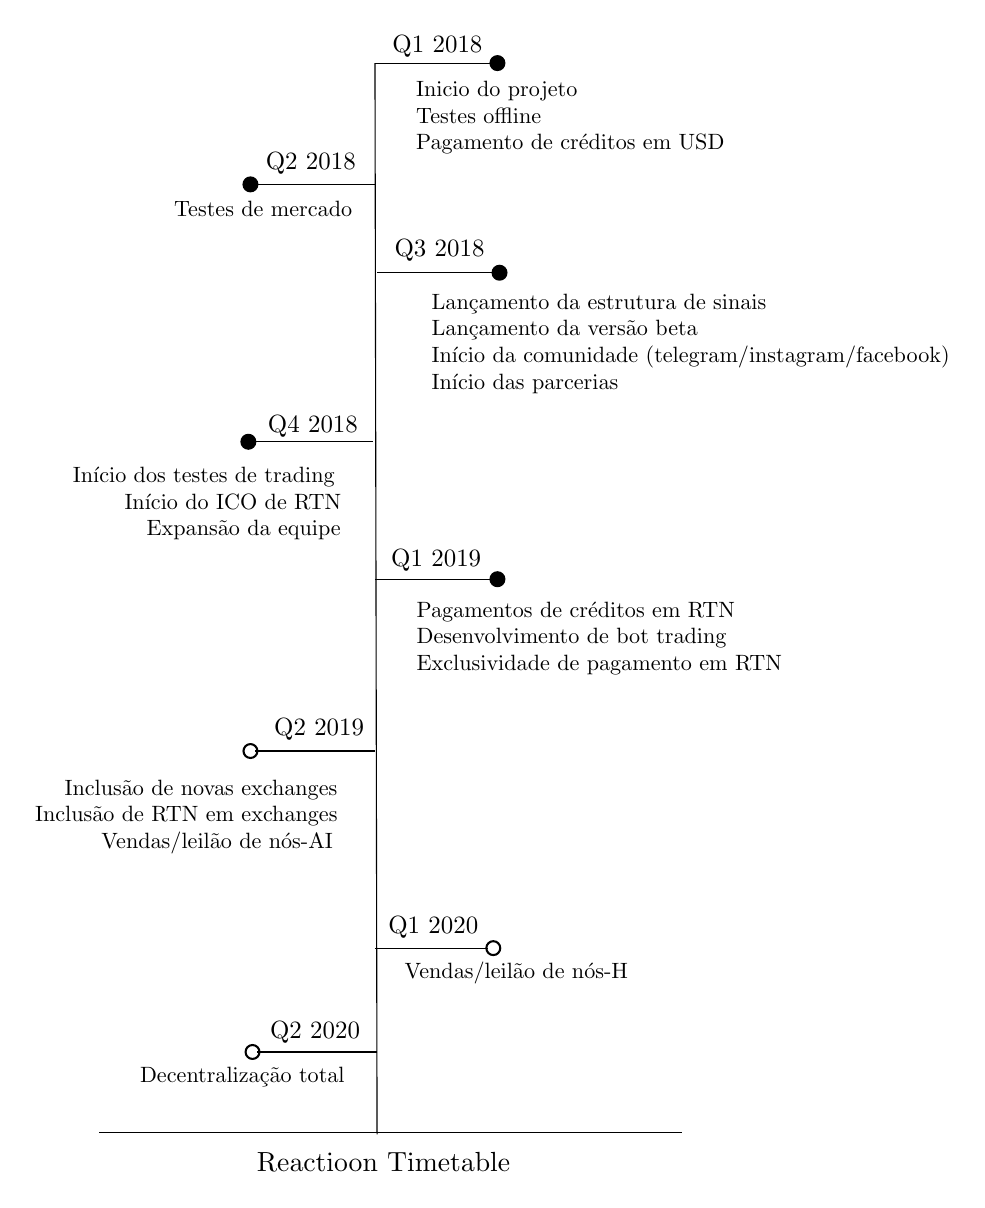
\begin{tikzpicture}[x=0.75pt,y=0.75pt,yscale=-1,xscale=1]
%uncomment if require: \path (0,600.9199981689453); %set diagram left start at 0, and has height of 600.9199981689453

%Straight Lines [id:da27949880366729407] 
\draw    (290.9,47.8) -- (291.9,563.92) ;


%Straight Lines [id:da016695516966388713] 
\draw    (290.9,47.8) -- (349.9,47.8) ;
\draw [shift={(349.9,47.8)}, rotate = 0] [color={rgb, 255:red, 0; green, 0; blue, 0 }  ][fill={rgb, 255:red, 0; green, 0; blue, 0 }  ][line width=0.75]      (0, 0) circle [x radius= 3.35, y radius= 3.35]   ;

%Straight Lines [id:da04938623797133035] 
\draw    (290.9,106.24) -- (230.9,106.24) ;
\draw [shift={(230.9,106.24)}, rotate = 180] [color={rgb, 255:red, 0; green, 0; blue, 0 }  ][fill={rgb, 255:red, 0; green, 0; blue, 0 }  ][line width=0.75]      (0, 0) circle [x radius= 3.35, y radius= 3.35]   ;

%Straight Lines [id:da10792958400592911] 
\draw    (290.9,379.24) -- (233.25,379.24) ;
\draw [shift={(230.9,379.24)}, rotate = 180] [color={rgb, 255:red, 0; green, 0; blue, 0 }  ][line width=0.75]      (0, 0) circle [x radius= 3.35, y radius= 3.35]   ;

%Straight Lines [id:da5389580478447318] 
\draw    (289.9,230.24) -- (229.9,230.24) ;
\draw [shift={(229.9,230.24)}, rotate = 180] [color={rgb, 255:red, 0; green, 0; blue, 0 }  ][fill={rgb, 255:red, 0; green, 0; blue, 0 }  ][line width=0.75]      (0, 0) circle [x radius= 3.35, y radius= 3.35]   ;

%Straight Lines [id:da7641576297357624] 
\draw    (291.9,148.8) -- (350.9,148.8) ;
\draw [shift={(350.9,148.8)}, rotate = 0] [color={rgb, 255:red, 0; green, 0; blue, 0 }  ][fill={rgb, 255:red, 0; green, 0; blue, 0 }  ][line width=0.75]      (0, 0) circle [x radius= 3.35, y radius= 3.35]   ;

%Straight Lines [id:da04724001416544876] 
\draw    (290.9,296.46) -- (349.9,296.46) ;
\draw [shift={(349.9,296.46)}, rotate = 0] [color={rgb, 255:red, 0; green, 0; blue, 0 }  ][fill={rgb, 255:red, 0; green, 0; blue, 0 }  ][line width=0.75]      (0, 0) circle [x radius= 3.35, y radius= 3.35]   ;

%Straight Lines [id:da9347215346833444] 
\draw    (290.9,474.2) -- (345.55,474.2) ;
\draw [shift={(347.9,474.2)}, rotate = 0] [color={rgb, 255:red, 0; green, 0; blue, 0 }  ][line width=0.75]      (0, 0) circle [x radius= 3.35, y radius= 3.35]   ;

%Straight Lines [id:da28779960793088244] 
\draw    (291.9,524.24) -- (234.25,524.24) ;
\draw [shift={(231.9,524.24)}, rotate = 180] [color={rgb, 255:red, 0; green, 0; blue, 0 }  ][line width=0.75]      (0, 0) circle [x radius= 3.35, y radius= 3.35]   ;

%Straight Lines [id:da8846097036360219] 
\draw    (158,563) -- (438.9,563) ;



% Text Node
\draw (385,74.02) node [scale=0.8] [align=left] {Inicio do projeto\\Testes offline\\Pagamento de créditos em USD};
% Text Node
\draw (290,55) node [scale=0.8] [align=left] {};
% Text Node
\draw (237,118) node [scale=0.8] [align=left] {Testes de mercado};
% Text Node
\draw (443,183) node [scale=0.8] [align=left] {Lançamento da estrutura de sinais\\Lançamento da versão beta\\Início da comunidade (telegram/instagram/facebook)\\Início das parcerias};
% Text Node
\draw (321,40) node [scale=0.9] [align=left] {Q1 2018};
% Text Node
\draw (260,96) node [scale=0.9] [align=left] {Q2 2018};
% Text Node
\draw (322,138) node [scale=0.9] [align=left] {Q3 2018};
% Text Node
\draw (261,223) node [scale=0.9] [align=left] {Q4 2018};
% Text Node
\draw (320.4,287.46) node [scale=0.9] [align=left] {Q1 2019};
% Text Node
\draw (264,369) node [scale=0.9] [align=left] {Q2 2019};
% Text Node
\draw (319,464.16) node [scale=0.9] [align=left] {Q1 2020};
% Text Node
\draw (262,515) node [scale=0.9] [align=left] {Q2 2020};
% Text Node
\draw (321,158) node [scale=0.8] [align=left] {};
% Text Node
\draw (210,260) node [scale=0.8] [align=left] {Início dos testes de trading\\ \ \ \ \ \ \ \ Início do ICO de RTN\\ \ \ \ \ \ \ \ \ \ \ Expansão da equipe};
% Text Node
\draw (399,325) node [scale=0.8] [align=left] {Pagamentos de créditos em RTN\\Desenvolvimento de bot trading\\Exclusividade de pagamento em RTN};
% Text Node
\draw (200,411) node [scale=0.8] [align=left] { \ \ \ \ Inclusão de novas exchanges\\Inclusão de RTN em exchanges\\ \ \ \ \ \ \ \ \ \   Vendas/leilão de nós-AI};
% Text Node
\draw (359,486) node [scale=0.8] [align=left] {Vendas/leilão de nós-H};
% Text Node
\draw (227,536) node [scale=0.8] [align=left] {Decentralização total};
% Text Node
\draw (295,577) node  [align=left] {Reactioon Timetable};


\end{tikzpicture}
}
\caption{Timetable diagram}
\end{figure}
\section{Token RTN}
O token RTN é utilizado dentro do ecossistema Reactioon e poderá ser negociado em exchanges nas quais estiver listado. Nós entendemos que o valor de cada token será proporcional aos lucros que os trading bots renderão aos investidores.

1 RTN corresponde a um crédito disponível na plataforma Reactioon. Atualmente cada crédito permite o uso do trading bot nos nós-AI por um dia por bitcoin movimentado. Nos nós-H os gestores serão responsáveis por definir a política de preços aplicáveis a cada nó, podendo ser por período, por volume ou por porcentagem sobre o ganho.

\subsection{ICO}
Nosso ICO será lançado dia 09/09/2018 e permanecerá ativo até o fim dos tokens RTN. O preço de cada RTN foi inicialmente definido em 1 USD, dado que atualmente os trading bots podem render até 5 \% ao mês. Entretanto, aos primeiros adeptos da plataforma será oferecido um desconto progressivo por lotes de venda.

Destaca-se que as etapas de desenvolvimento do projeto são independentes do ICO, mas que o ICO é a forma de financiamento da equipe de desenvolvimento, ou seja, quanto mais o projeto é financiado mais rápido é desenvolvido, podendo sofrer alterações na Timetable atual. 

A tabela a seguir apresenta os descontos progressivos e o número de tokens oferecidos no ICO do projeto.
\begin{table}[!h]
        \centering
        
\begin{tabular}{p{0.2\textwidth}p{0.2\textwidth}|p{0.2\textwidth}}
\begin{center}
\textbf{De}
\end{center}
 & \begin{center}
\textbf{Até}
\end{center}
 & \begin{center}
\textbf{Preço do token durante ICO}
\end{center}
 \\
\hline 
 \begin{center}
{\small 0}
\end{center}
 & \begin{center}
{\small 100,000}
\end{center}
 & \begin{center}
{\small USD 0.25}
\end{center}
 \\
\hline 
 \begin{center}
{\small 100,000}
\end{center}
 & \begin{center}
{\small 500,000}
\end{center}
 & \begin{center}
{\small USD 0.50}
\end{center}
 \\
\hline 
 \begin{center}
{\small 500,000}
\end{center}
 & \begin{center}
{\small 1,000,000}
\end{center}
 & \begin{center}
{\small USD 0.75}
\end{center}
 \\
\hline 
 \begin{center}
{\small 1,000,000}
\end{center}
 & \begin{center}
{\small 3,000,000}
\end{center}
 & \begin{center}
{\small USD 1.00}
\end{center}
 \\

\end{tabular}
        \end{table}


\subsection{Airdrops}
Airdrops de RTN serão disponibilizados a cada nova listagem em exchanges.
\subsubsection{Token division}
A distribuição do token RTN segue o seguinte plano:
\begin{itemize}
    \item [] Fundadores: 3,000,000
    
    \item [] ICO: 3,000,000

    \item [] Cold Wallet: 15,000,000

    \item [] Total emitido: 21,000,0000

\end{itemize}

\section{Conclusão}

Nós da Reactioon pretendemos mudar o paradigma de gestão de fundos no contexto global. Nós acreditamos que o nosso modelo representa uma forma flexível e transparente para gerenciamento de fundos atuais e futuros negociados através de contratos inteligentes. Nossa estrutura poderá ser utilizada para gestões de fundos independentemente do volume, de forma segura para o cliente e rentável para o gestor.

A proposta da Reactioon está em constante aperfeiçoamento e seguindo as práticas de mercado. Buscamos ser uma alternativa democrática e moderna aos fundos de investimento sem transparência e sem gestão ativa. Acreditamos que a adoção da plataforma por investidores irá gradativamente atrair bons gestores de fundos tradicionais. Além disso, acreditamos que a medida que o lastro de ativos atuais for emitido em contratos inteligentes a plataforma irá se expandir.

Se você compartilha da nossa filosofia e acredita no futuro da tecnologia blockchain, nós te convidamos a se tornar um investidor do projeto e a compartilhar nossos serviços. Nós estamos apenas começando uma jornada de grande mudança. Venha com a gente!

Reactioon: O futuro é agora!

% Tabelas devem ser centradas na página e numeradas com algarismos arábicos.  A legenda deve ficar acima da tabela.   Linhas verticais são opcionais.  Separe a figura do texto anterior com um espaço de 12 pt. 

%\section{Equações}

%Equações devem separadas do texto por espaços de 6 pt (meia linha) antes e depois.  Numere as equações com algarismos arábicos, colocados entre parênteses e alinhados à esquerda,  como mostra o exemplo a seguir.

%\begin{equation}
%x = y+1.
%\end{equation}

%Pontue a equação e continue o texto seguinte como se a equação fosse parte do texto.  Por exemplo, a equação 1 termina com um ponto final e o parágrafo seguinte a ela (que é este) começa em maiúscula e com tabulação.  Segundo exemplo: em

%\begin{displaymath}
%y = x-1,
%\end{displaymath}

%segue-se a equação 2 com uma vírgula, e o parágrafo seguinte (que é este) começa em minúscula e sem tabulação. Utilize "\$"  para inserir equações no meio do texto, como em $y=x-2$.

%\section{Referências Bibliográficas}

%Referências devem ser citadas no texto no formato (SOBRENOME, ano) ou (SOBRENOME1 e SOBRENOME2, ano), entre parênteses, com os sobrenomes dos autores em maiúscula e o ano de publicação com 4 dígitos.  Havendo muitos autores, indique o primeiro e abrevie os demais com “et al.” – por exemplo (FULANO et al., 1998).

%Caso deseje citar uma obra forma textual no artigo, inclua o ano da publicação entre parênteses após o(s) nome(s) dos autor(es).  Por exemplo: “Segundo Fulano e Sicrano (1999), é possível que...”.

%Para mais informações sobre como citar adequadamente diferentes tipos de trabalho, consulte por exemplo as diretrizes compiladas pela Divisão de Bibliotecas da Escola Politécnica da USP (2013), disponível em

%http://www.poli.usp.br/images/stories/media/download/bibliotecas/DiretrizesTesesDissertacoes.pdf

%\appendix
%\section*{Apêndices}
 
%A seção de apêndices é opcional.  Se precisar incluí-la, deixe 24 pt (duas linhas) de espaço antes do título “Apêndices”,  escrito centrado na linha, em letras maiúsculas (ou versalete) e tamanho 14 pt.
 
%\addcontentsline{toc}{section}{Apêndices}   % Definindo seção de apêndice
%\renewcommand{\thesection}{\textit{\Alph{section}} }
%\section{\textit{Primeiro apêndice}}
 
%Deixe um espaço de 12 pt antes e depois do título do apêndice.  Escreva o título em tamanho 14 pt e em itálico.  Os apêndices devem ser numerados com letras maiúsculas.


%\section*{Agradecimentos}

%Agradecimentos (opcional).  Deixe um espaço de 24 pt antes do título “Agradecimentos”, escrito centrado na linha, em maiúscula (ou versalete) e tamanho 14 pt.  Escreva o texto dos agradecimentos após um espaço de 12 pt.

% \centering\section*{REFERENCES}
%O título da seção de referências deve ter um espaço antes de 24 pt e deve ser escrito centrado na linha, em maiúscula (ou versalete) e tamanho 14 pt.  Deixe um espaço de 12 pt antes do texto da primeira referência.  Deixe um espaço de 6 pt (meia linha) entre as referências.

%Liste as obras pela ordem alfabética do sobrenome do primeiro autor (ou nome da empresa).  Não numere as referências.  Alguns exemplos:

%\noindent SOBRENOME, Nome. Título da publicação.  Edição, Cidade de publicação: Editora, ano, páginas $\{ $Referencia$\} $.

%\noindent SOBRENOME1, Nome1;  SOBRENOME2, Nome2.  Título da publicação.  Edição, Cidade de publicação: Editora, ano, páginas.

%\noindent SOBRENOME1, Nome1;  SOBRENOME2, Nome2; et al.  Título da publicação.  Edição, Cidade de publicação: Editora, ano, páginas.

%Também é possível utilizar o comando \textbackslash bibliography\{\} do LaTeX para inserir as referências a partir de um arquivo .bib, como mostrado a seguir. Para as referências presentes no arquivo .bib aparecerem nessa seção, elas devem ter sido citadas em algum ponto do artigo com o comando \textbackslash cite\{\}, como a seguir: \cite{referencia1}, \cite{referencia2} e \cite{referencia3}.

%\vspace{-8mm}
\begingroup
\makeatletter
\renewcommand{\chapter}{\@gobbletwo}
\makeatother
\bibliographystyle{abntex2-alf-mod}
\bibliography{mybibfile}
\endgroup

%(Se seu artigo não for escrito em inglês, acrescente aqui as versões em inglês do título, resumo e palavras-chaves)

%\begin{changemargin}{1cm}{1cm} 

%Title: Template for Papers of the Mecatrone Journal 

%\textbf{Abstract} – This is the English version of the resume.

%\textbf{Keywords} – Comma separated list of keywords.

%\end{changemargin}

% \begin{figure}[h]
%     \includegraphics[width=0.5\textwidth]{figure2}
%     \caption{figura2}
%     \label{figura2}
% \end{figure}
\textbf{José Wilker}, Criador da tecnologia do Reactioon. Faz tudo. programador PHP / Javascript / NodeJS / C / ShellScript com habilidades em gerenciamento de projetos e Linux. Gosta de  Matemática, Xadrez, Cartas e jogos de RPG/Estratégia.

\textbf{Jonathas Marcelo Pereira Figueiredo}, Graduado em Engenharia Mecatrônica na Escola Politécnica da Universidade de São Paulo (POLI-USP), Brasil. Graduado em Sistemas Autônomos e Engenharia da Informação na ENSE3 Grenoble-INP, França.

\textbf{Lucas Tonini}, Especialista em Marketing com experiência em gestão para campanhas digitais.


% \begin{figure}[h]
%     \includegraphics[width=0.5\textwidth]{figure2}
%     \caption{figura2}
%     \label{figura2}
% \end{figure}



\end{document}